\begin{figure}
	\begin{center}
	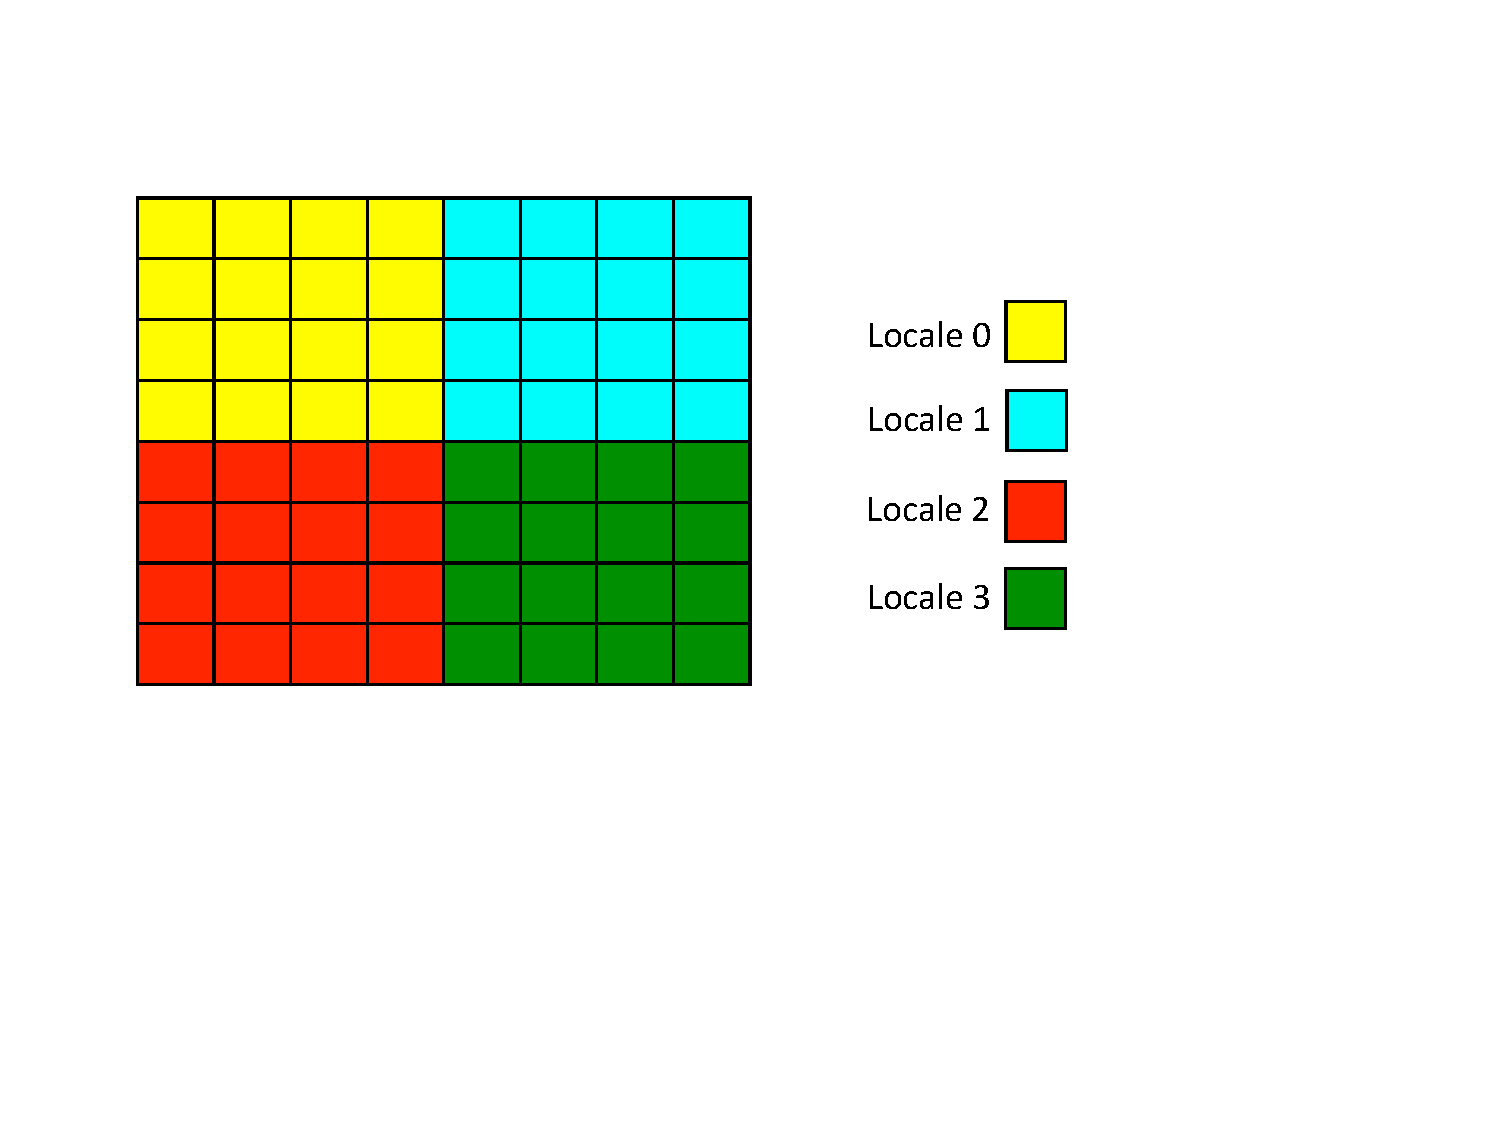
\includegraphics[scale=0.55]{./Figures/block_dist}
	\caption{Chapel Block distribution.}
	\label{block_dist}
	\end{center}
\end{figure}

\section{Chapel's Data Distributions}\label{sec:data_distributions} 

Figures \ref{block_dist} - \ref{block_cyc_dist} illustrate the Chapel data distributions that we explored in this work: Block, Cyclic, and Block Cyclic. Each figure shows how a two-dimensional 8 x 8 array can be distributed in Chapel using each distribution. Figure \ref{block_dist} illustrates the Block distribution. Elements of the array are mapped to locales evenly in a dense manner. In Figure \ref{cyc_dist}, the Cyclic distribution, elements of the array are mapped in a round-robin manner across locales. Finally, in Figure \ref{block_cyc_dist} the Block Cyclic distribution is shown. Here, a number of elements specified by a block size parameter is allocated to consecutive array indices in a round-robin fashion. In Figure \ref{block_cyc_dist}, the distribution takes in a 2 x 2 block size parameter. Further details about Block, Cyclic, and Block Cyclic distributions in Chapel are described in \cite{distributions}.

The choice of data distribution to use for a program boils down to computation and communication efficiency. Different programs and architectures may require different data distributions. It has been shown that finding an optimal data distribution for parallel processing applications is an NP-complete problem, even for one- or two-dimensional arrays \cite{mace1987memory}. Certain program data access patterns will result in fewer communication calls if the data is distributed in a particular way. For example, many loops in stencil programs that contain nearest neighbor computation will have better communication performance if the data is distributed using a Block distribution. This occurs because on a given loop iteration, the elements accessed are near each other in the array and therefore are more likely to reside on the same locale block. Accessing elements on the same block does not require a remote data access and can be done faster. However, programs that access array elements far away from each other will have better communication performance if data is distributed using a Cyclic distribution. Here, a Block distribution is almost guaranteed to have poor performance because the farther away accessed elements are the more likely they reside on different locales. 

\begin{figure}
	\begin{center}
	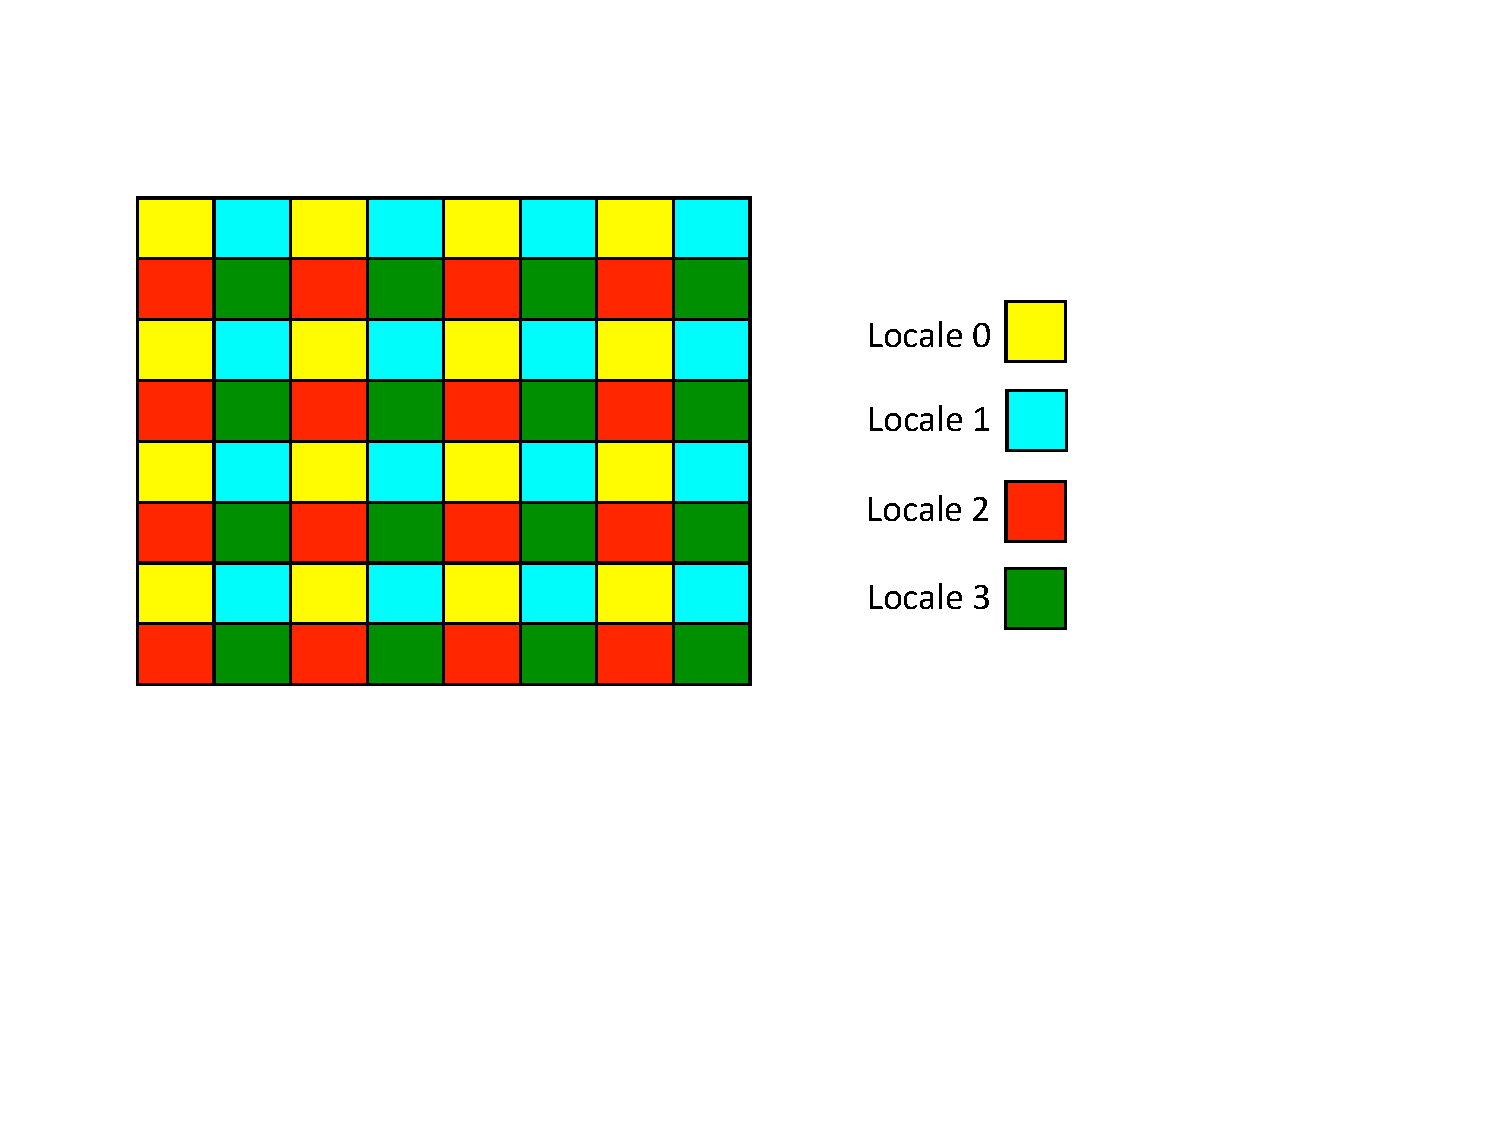
\includegraphics[scale=0.55]{./Figures/cyc_dist}
	\caption{Chapel Cyclic distribution.}
	\label{cyc_dist}
	\end{center}
\end{figure}

\begin{figure}
	\begin{center}
	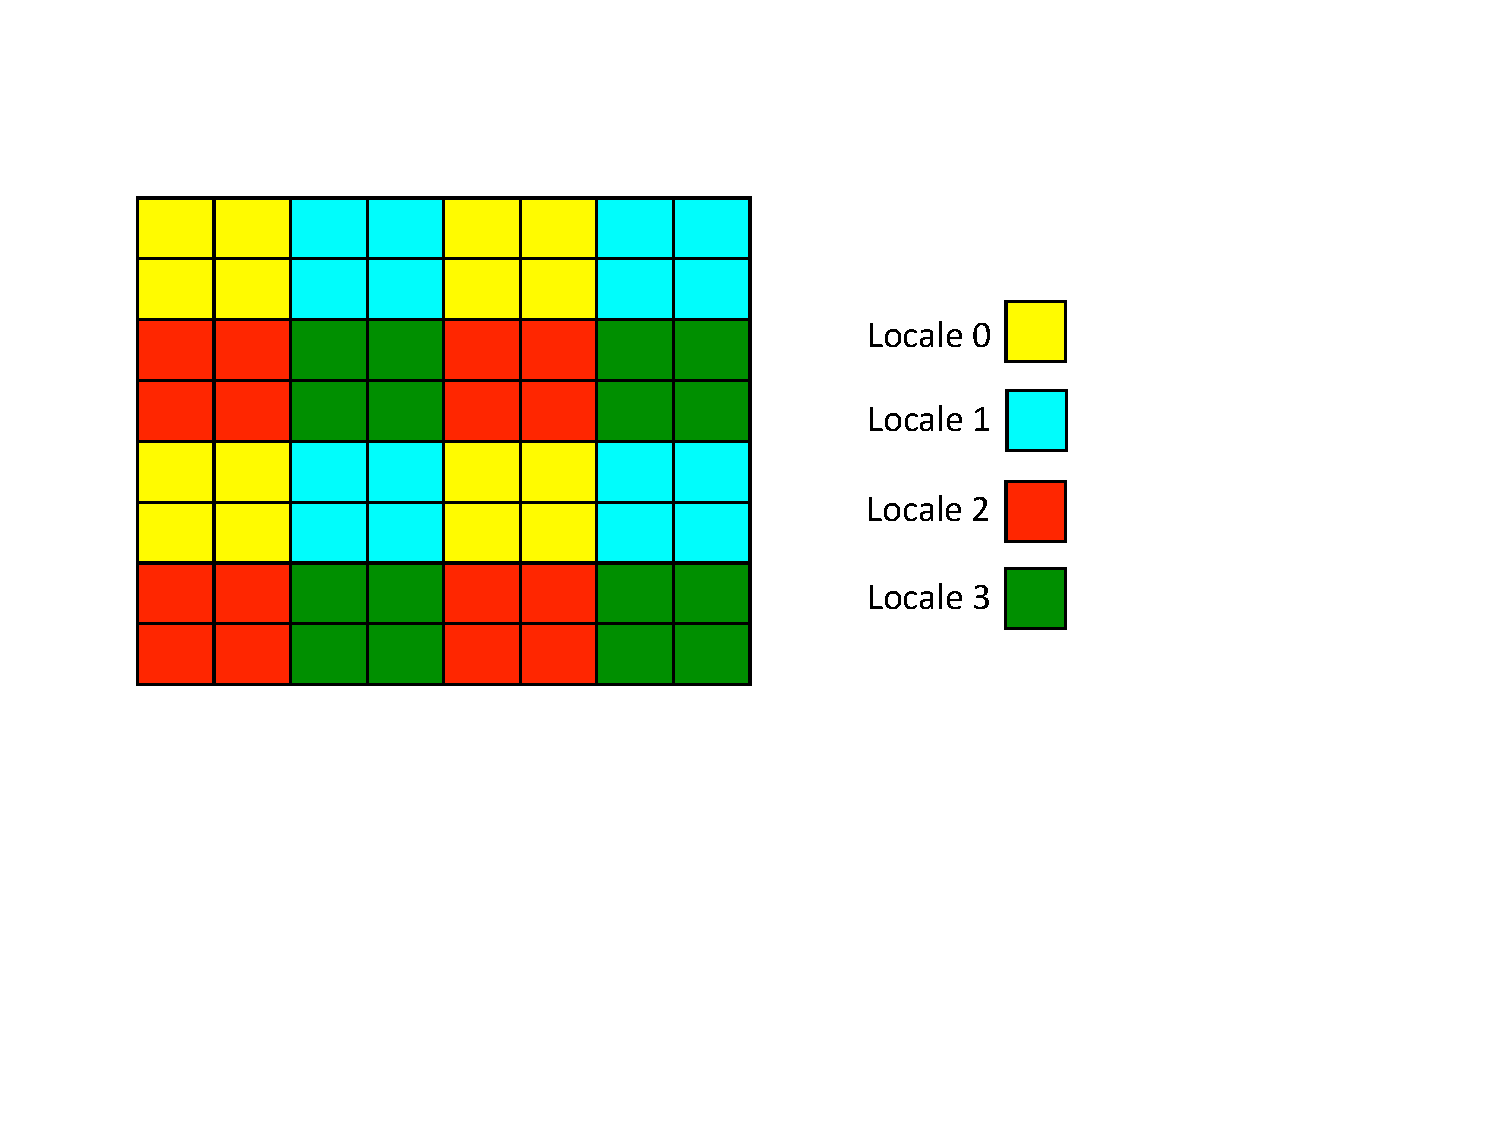
\includegraphics[scale=0.55]{./Figures/block_cyc_dist}
	\caption{Chapel Block Cyclic distribution with a 2 x 2 block size parameter.}
	\label{block_cyc_dist}
	\end{center}
\end{figure}

A programmer may choose a particular data distribution for reasons unknown to the compiler. These reasons may not even take communication behavior into account. For example, Cyclic and Block Cyclic distributions provide better load balancing of data across locales than a Block distribution when array sizes may be changed dynamically because in Cyclic and Block Cyclic distributions, the locales of existing array elements do not change when new array elements are added at the end of the array. In many applications, data redistribution may be needed if elements of a data set are inserted or deleted at the end of the array. In particular, algorithms to redistribute data using a new block size exist for the Block Cyclic distribution \cite{prylli1997fast,walker1996redistribution}. If an application uses a dynamic data set with elements that are appended, a Cyclic or Block Cyclic distribution is superior to Block because new elements are added to the locale that follows the cyclic or block-cyclic pattern. For Block, the entire data set would need to be redistributed every time a new element is appended, which can be expensive. 

Compatibility with other PGAS languages might be an important consideration for a programmer when selecting a data distribution. Data sets used by Chapel programs and other PGAS programs should use Cyclic or Block Cyclic distributions because other PGAS languages may not support the Block distribution. A programmer would benefit by distributing the same data set using only one scheme so the data would not have to be replicated for different programs. This is an important consideration for vast data sets which have already been distributed on message passing computers, and we want to perform additional computation on them, perhaps with other programs.  

Therefore in this work, it is our view that the compiler should not change the programmer's choice of data distribution in order to achieve better runtime and communication performance. The compiler should attempt to perform optimizations based on the data distribution that the programmer specified. Our optimization is meant to be applied whenever the programmer specifies a Cyclic or Block Cyclic distribution. It is not applied when the programmer specifies a Block distribution.